% 
% Annual Cognitive Science Conference
% Sample LaTeX Paper -- Proceedings Format
% 

% Original : Ashwin Ram (ashwin@cc.gatech.edu)       04/01/1994
% Modified : Johanna Moore (jmoore@cs.pitt.edu)      03/17/1995
% Modified : David Noelle (noelle@ucsd.edu)          03/15/1996
% Modified : Pat Langley (langley@cs.stanford.edu)   01/26/1997
% Latex2e corrections by Ramin Charles Nakisa        01/28/1997 
% Modified : Tina Eliassi-Rad (eliassi@cs.wisc.edu)  01/31/1998
% Modified : Trisha Yannuzzi (trisha@ircs.upenn.edu) 12/28/1999 (in process)
% Modified : Mary Ellen Foster (M.E.Foster@ed.ac.uk) 12/11/2000
% Modified : Ken Forbus                              01/23/2004
% Modified : Eli M. Silk (esilk@pitt.edu)            05/24/2005
% Modified : Niels Taatgen (taatgen@cmu.edu)         10/24/2006
% Modified : David Noelle (dnoelle@ucmerced.edu)     11/19/2014

%% Change "letterpaper" in the following line to "a4paper" if you must.

\documentclass[10pt,letterpaper]{article}

\usepackage{cogsci}
\usepackage{comment}
\usepackage{pslatex}
\usepackage{apacite}
\usepackage{amsmath,amssymb}
\usepackage{graphicx}
\usepackage{subcaption}
\usepackage{color}
\usepackage{url}
\usepackage{todonotes}
\usepackage{mathtools}
\usepackage{stmaryrd}
\usepackage{booktabs}
\usepackage{array}
\usepackage{caption}
\usepackage{subcaption}
\usepackage[export]{adjustbox}


\newcommand{\jefan}[1]{{\color{blue}{[jefan: #1]}}}
\newcommand{\kushin}[1]{{\color{orange}{[kushin: #1]}}}

\title{Semantic structure in communicative drawings}
 
% \author{\begin{tabular}[htbp]{c@{\extracolsep{1em}}c@{\extracolsep{1em}}c@{\extracolsep{1em}}c} \\
% {\large \bf Kushin Mukherjee} & {\large \bf Robert X. D. Hawkins} & {\large \bf Judith E. Fan}\\
% Department of Cognitive Science  & Department of Psychology & Department of Psychology \\ 
% Vassar College & Stanford University & Stanford University \\
% \texttt{kumukherjee@vassar.edu} & \texttt{rxdh@stanford.edu} & \texttt{jefan@stanford.edu} \\
% \end{tabular}
% }

\author{{\large \bf Kushin Mukherjee\textsuperscript{1}, Robert X. D. Hawkins\textsuperscript{2}, Judith E. Fan\textsuperscript{2,3}} \\
\textsuperscript{1}Department of Cognitive Science, Vassar College, \\
\textsuperscript{2}Department of Psychology, Stanford University, \\
\textsuperscript{3}Department of Psychology, University of California, San Diego}


\begin{document}

\maketitle 

\begin{abstract}
Drawing is a versatile tool for communication, spanning detailed renderings and sparse sketches. 
Even the same object can be drawn in different ways, depending on the context. 
Here we examine the semantic structure of object drawings to understand how people deploy perceptual information and conceptual knowledge to convey relevant information in context.
Towards this end, we developed a web-based platform to densely annotate drawings of real-world objects produced in different semantic contexts, including detailed and simpler sketches of each object. 
We found that: \textit{1}, people are highly consistent in how they interpret what individual strokes represent; \textit{2}, single strokes tend to correspond to single parts; \textit{3}, strokes representing the same part tend to be clustered in time; and \textit{4}, detailed and sparse drawings of the same object emphasized similar part information, although \textit{5}, detailed drawings of different objects tend to be more distinct from one another than simpler ones. 
Taken together, our results support the notion that during visual communication, people readily deploy their abstract understanding of the semantic structure of objects in order to select actions that effectively communicate about them. 
More broadly, they highlight the importance of structured knowledge for understanding how pictorial representations convey meaning. 


% We found that: (1) people are highly consistent in how they interpret what individual strokes mean; (2) single strokes tend to represent a single part category (e.g., leg vs. leg + seat), while multiple strokes may be combined to represent an entire part category (e.g., all the legs on a chair); and (3) strokes representing the same part tend to be clustered in time, suggesting that people tend to start and finish drawing one part of an object before moving onto the next.

\textbf{Keywords:} 
sketch understanding; perceptual organization; visual production; object representation; pragmatics
\end{abstract}

\section{Introduction}
This is where our introduction will go.

\section{Methods}

\subsection{Dataset}

We required sketches of common objects created under different contexts. 
So we obtained sketch data from a two-player 'Pictionary'-style reference game experiment. 
In this experiment, a 'sketcher' aimed to produce sketches of target objects to distinguish them from three distractor objects. 
A 'viewer' had to guess which of the 4 images the sketch represented. 
The targets and distractors were chosen from a set 32 real-world objects belonging to 4 basic-level categories: cars, chairs, dogs, and birds. 
Each category had 8 distinct exemplars. 
There were 2 main context conditions in this experiment - close and far. 
In the close condition, the target image and the distractors belonged to the same basic-level category. 
In the far condition, the target and each of the distractors belonged to a different basic-level category.

We obtained 1198 sketches for the annotation task. 
These sketches were represented as scalable vector graphics (SVG) images. 
The strokes that participants made on the canvas when creating the sketch can be represented as a concatenated string of cubic Bezier curves.  
Thus, the final sketch can be represented by a list of such concatenated strings, each of which corresponds to an event of the participant placing their drawing instrument on the canvas, making some marks on the canvas, and lifting the instrument off of the canvas. 
We were interested in collecting fine-grained annotations of these strokes, so we split strokes into sub-stroke elements, which we called splines. 
A single spline was equivalent to a single cubic Bezier curve, i.e., a Bezier curve with two fixed end points and two control points to control curvature. 
We had participants in our annotation task label each sketch's constituent splines.


\subsection{Participants}

We recruited a total of 326 participants via Amazon Mechanical Turk (AMT).  
For this experiment, participants provided informed consent in accordance with the Stanford University IRB. 
Participants were paid a base amount of \$0.35 and were given an additional bonus of \$0.002 for every stroke they annotated. 
In addition to this, they were given a \$0.02 bonus for every sketch for which they labeled all strokes. 

\subsection{Annotation Procedure}

To collect fine-grained annotations of our sketches, we implemented a web-based Javascript annotation tool. 
Each participant annotated 10 sketches. 
We provided participants with a sketch to be annotated on a canvas as well as a category-specific menu of labels, which they were encouraged to use for the annotation task. We also provided them with the option of entering their own labels through a free-response box. 
The original set of images the sketcher had to discriminate between were shown to help the annotator better understand the contents of the sketch.
Labeling was done by clicking on individual splines or clicking and dragging across multiple splines to highlight them before assigning them a label.
Participants were encouraged to conduct their labeling of strokes in bouts — they were to highlight all the strokes corresponding to a single instance of a part before selecting a label from the menu. 
Participants could do the task at their own pace and continue to a subsequent sketch whenever they felt they were ready. 
They could choose to continue to the next trial without labeling every stroke in a sketch, but they would lose out on the completion bonus as well as the amount they would have earned for labeling the remaining strokes.
\noindent In total, we collected 3608 annotations of 1195 unique sketches. 

\subsection{Preprocessing}
After collecting annotations, we filtered out any sketches that didn't have all of its constituent splines labeled. This left us with 3319 annotations of 1190 unique sketches.
Since there was some variability in the number of times each sketch in our dataset was annotated, we selected those sketches that had been annotated exactly 3 times. This left us with 764 unique sketches, each of which had been annotated 3 times.
We also created unique dictionaries for each object category that mapped participant-generated labels to the most frequently occurring labels in our dataset. This helped reduce the total number of unique labels in our dataset from 228 to 24.

Given that our goal was to created an annotated dataset of sketches created under different contexts, we required that the annotations we collected through our interface be reliable. In order to assess this reliability, we looked at whether different annotators saw the same parts in these abstract sketches of objects. Specifically, we looked at inter-annotator reliability in spline labels between participants for each spline in our dataset. Reliability was measured in terms of 'agreement' on spline labels. For example, a 3/3 agreement score for a given spline meant that each of the 3 annotators applied the same label to that spline. We found that 67.85\% of splines in our dataset had 3/3 inter-annotator agreement, 27.77\% of splines had 2/3 agreement, and 4.38\% of splines had no agreement, which means that each participant applied a different label for each of those splines.
For the purposes of analysis, we set the modal label for each spline as its true label.

\section{Results}

\subsection{Relationship between strokes and parts}

\begin{figure}[htbp]
\centering
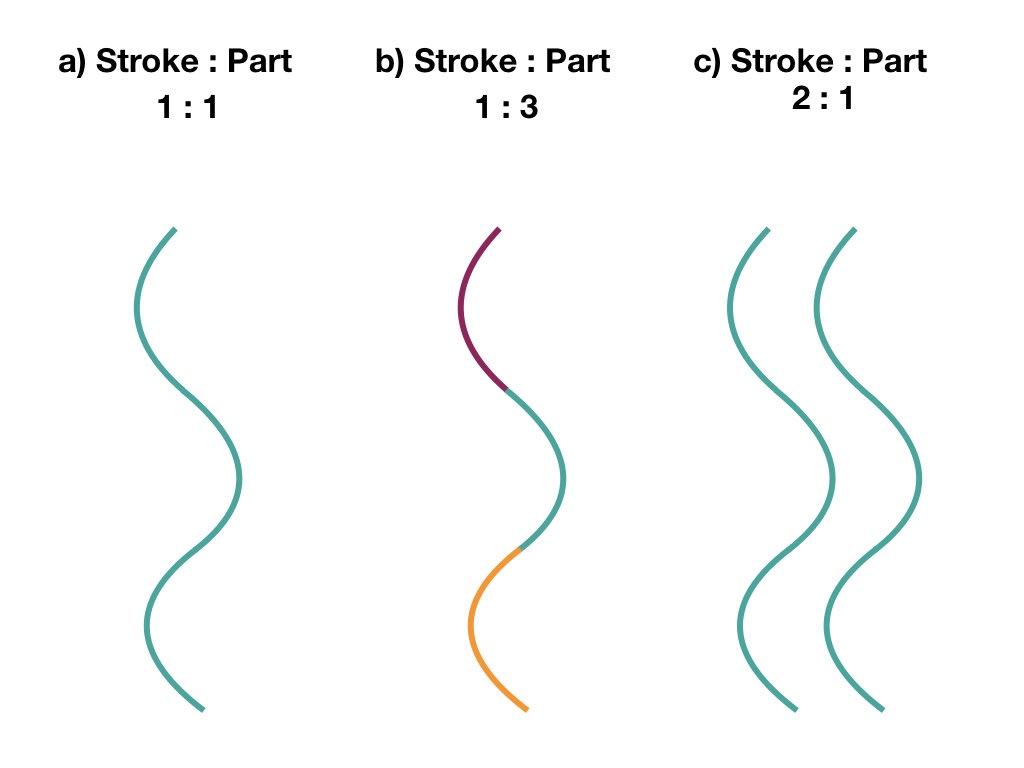
\includegraphics[width=0.5\textwidth]{figures/Part-Stroke.jpeg}
\caption{The three part-stroke relationships we explored. Each squiggle represents a hypothetical stroke. Different colors indicate different part-labels.}
\end{figure}

\begin{figure}[htbp]
\begin{subfigure}[t]{0.2\textwidth}
\centering
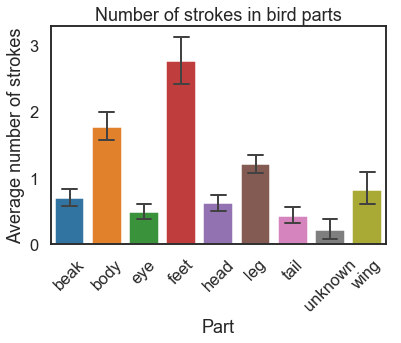
\includegraphics[width=1.2\textwidth]{figures/bird_average_parts.png}
\caption{Bird}
\end{subfigure}
 \hfill
\begin{subfigure}[t]{0.2\textwidth}
\centering
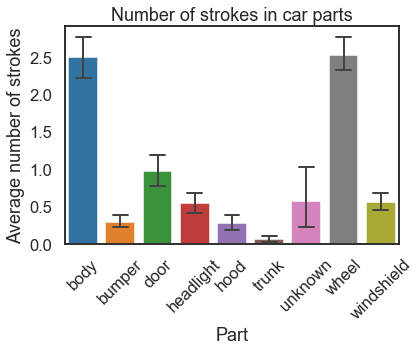
\includegraphics[width=1.2\textwidth]{figures/car_average_parts.png}
\caption{Car}
\end{subfigure}
\hfill
\begin{subfigure}[t]{0.2\textwidth}
\centering
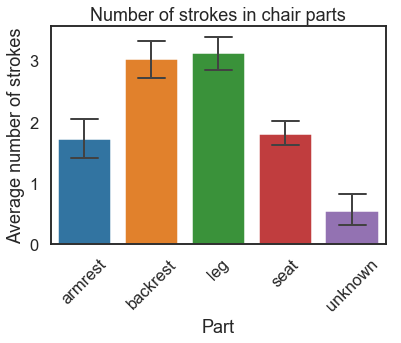
\includegraphics[width=1.2\textwidth]{figures/chair_average_parts.png}
\caption{Chair}
\end{subfigure}
 \hfill
\begin{subfigure}[t]{0.2\textwidth}
\centering
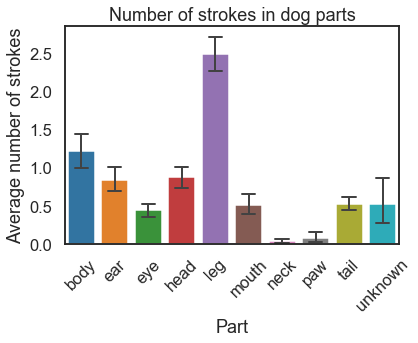
\includegraphics[width=1.2\textwidth]{figures/dog_average_parts.png}
\caption{Dog}
\end{subfigure}
\caption{Average number of strokes used to draw each part per category. While participants use multiple strokes to represent some parts, other parts are sometimes expressed using single strokes.}
\label{strokesperpart}
\end{figure}


People's hierarchical organization of visual concepts, such object category membership being determined by its constituent parts, allows for robust recognition of objects in the real world. 
We were interested in whether people might employ similar abstractions in producing sketches of such objects as well. 
Since an individual stroke correspond to a person's decision to make a mark on the canvas, we looked at the relationship between strokes and the parts that they represented in our dataset. 
We explored 3 possible stroke-to-part relationships:
a) Singular strokes correspond to singular parts, b) Singular strokes are used to convey multiple parts, that is, strokes cross semantic boundaries, and c) Multiple strokes are required to convey a single part. 

We compared a) and b) by looking at within-stroke label agreement for spline labels for all strokes in our dataset. High agreement among all the splines in a given stroke would be indicative of that being used to represent a single part. 
On the other hand, low agreement would indicate that stroke crosses semantic boundaries and is used to represent different parts. 
We found that splines contained in 76.85\% of strokes in our dataset shared a single label, 12.75\% of strokes contained 2 labels, and less than 11\% of strokes contained 3 or more labels. 
People, in general, tended to use their strokes to draw a single part while only sometimes utilizing a single stroke to represent multiple parts.

We also compared a) and c) by looking at the average number of strokes used to represent specific parts within a given category of sketches. 
A high average number of strokes for a given part would indicate that multiple strokes are utilized to draw that part, whereas a low average would indicate that a single or few strokes might suffice in depicting that part. 
Figure \ref{strokesperpart} shows these part-specific stroke averages by object category.
\kushin{I feel the above summary, including the figure caption for figure 2 is a little inconclusive. Thoughts on how to remedy this?}

\subsection{Stroke sequence organization}

\begin{figure}
\centering
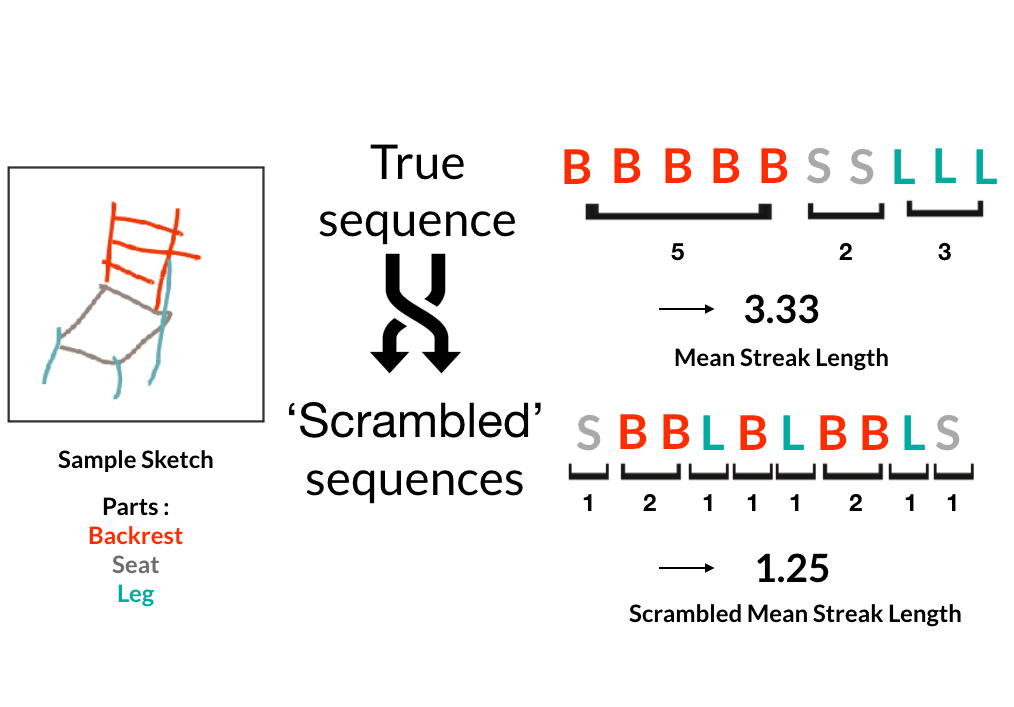
\includegraphics[width=0.5\textwidth]{figures/Part_sequence.png}
\caption{Analyzing stroke sequences in sketches. We first coded each stroke in our dataset in terms of its part label. Whenever multiple consecutive strokes that the sketcher had made shared a part-label, we counted the number of such strokes and termed it as a streak length for that part. This process was repeated for every stroke in a given sketch, after which we averaged over all the streak lengths for every part to obtain a single mean streak length value for every sketch in our dataset. To test whether strokes of the same part were reliably being drawn in bunches we scrambled the order of strokes in each sketch and calculating a 'scrambled' mean streak length. We repeated this scrambling process 1000 times to get a distribution of scrambled mean streak lengths for every sketch.}
\label{stroke_sequence_fig}
\end{figure}

Since individual strokes seemed to mostly correspond to singular part labels, we can view strokes as the building blocks for sketches much like words are the building blocks for sentences. Under this view of stroke organization, we looked at whether there was any meaningful temporal organization of strokes in terms of their part labels. If there was any such organization, any variation between the context conditions would also highlight a difference in how parts are mapped onto strokes under different communicative needs. This investigation was done through a permutation test approach where we created distributions of scrambled stroke sequences to test whether in the true sequence strokes of the same part were preferentially grouped together. Figure \ref{stroke_sequence_fig} outlines the procedure we undertook for this analysis.
74 sketches were excluded from this analysis because a) they consisted of only a single stroke, b) all the constituent strokes shared the same part label, or c) each stroke in the sketch had a unique label, making the permutation procedure not feasible.
We calculated the z-score of the true sequence of every sketch relative to their scrambled distributions. The higher this statistic was, the greater the amount of grouping of similar parts was relative to if the strokes were organized in a random fashion.

 The mean z-score for sketches in the close condition was 2.58 (95 CI: 2.26, 2.90) and 1.56 (95 CI: 1.38, 1.74) for the far condition.


 
 


% table for now: Is there spatial contiguity in how people structure their sketches?

\subsection{Modulation between communicative contexts}
\jefan{where we would report analysis of the sketch part features (num strokes, arc length)
e.g., when the far sketches are more abstract, how does that manifest in this feature representation?
like, are they more similar to each other, more like "bird" and lacking object-specific details?
a way of measuring this is that the centroid (euclidean norm, magnitude of the vector) is closer to the origin for far vs. close, and also that the RMSD to centroid of far sketches is smaller than for close sketches.... }


\section{Discussion}

\section{Acknowledgments}

\subsection{Tables}

\subsection{Figures}






\section{References}

\bibliographystyle{apacite}

\setlength{\bibleftmargin}{.125in}
\setlength{\bibindent}{-\bibleftmargin}

\bibliography{CogSci_Template}


\end{document}
